\documentclass[10pt,a4paper]{article}
\usepackage[margin=2.2cm]{geometry}
\usepackage[T1]{fontenc}
\usepackage{amsmath,amssymb,amsthm,mathtools}
\usepackage{booktabs,longtable,array}
\usepackage{enumitem}
\usepackage{xcolor}
\usepackage{algorithm}
\usepackage{algpseudocode}
\usepackage{tikz}
\usetikzlibrary{positioning,arrows.meta}
\usepackage{hyperref}
\hypersetup{colorlinks=true,linkcolor=blue!50!black,pdftitle={Summary of the proof}}

\setlength{\parindent}{0pt}
\setlength{\parskip}{0.45em}
\setlist{topsep=0.3em,itemsep=0.2em}
\renewcommand{\arraystretch}{1.25}

\newtheorem*{result}{Result}

\newcommand{\E}{\mathbb{E}}
\DeclareMathOperator{\Prob}{Pr}
\DeclareMathOperator{\Sol}{Sol}
\DeclareMathOperator{\dist}{dist}
\newcommand{\Lp}{\mathcal{L}}
\newcommand{\SAT}{\text{ SAT}}
\newcommand{\Hyp}{\textup{(H)}}

% column types for the symbol tables
\newcolumntype{S}{>{\raggedright\arraybackslash}p{0.19\textwidth}}
\newcolumntype{M}{>{\raggedright\arraybackslash}p{0.56\textwidth}}
\newcolumntype{W}{>{\raggedright\arraybackslash}p{0.17\textwidth}}

\title{\bfseries Summary of\\ ``The \(3/2\) Phase Transition in Semi-Random 2-SAT''}
\date{}

\begin{document}
\maketitle
\vspace{-2.5em}

\noindent This summary is a reading aid for Section 1 of the paper. It first
collects the symbols by scope, and then follows Section 1 in order: the graph
reduction (Section 1.4), the deletion experiment (Section 1.5), and the
analysis for difficult graphs (Section 1.6). All numbers (Lemma 2.5,
Theorem 1.12, \dots) refer to the current \texttt{main.pdf}.

%======================================================================
\section{Symbol table}\label{sec:symbols}
%======================================================================

The symbols are sorted like variables in a program. \emph{Global} symbols are
defined in Section 1 and are valid in the whole paper, \emph{module} symbols are
valid only in one section (Section 4 and Appendices A, B count as one module),
and \emph{local} symbols live inside one proof. Some global symbols are
\emph{parameters}, like the arguments of a function: a lemma that begins with
``Fix \(\Delta,R,\rho\)'' holds for all values, and a later proof calls it with
particular values, for example \(R=R_0\).

\subsection{Global symbols (Section 1, valid everywhere)}

\begin{longtable}{SMW}
\toprule
Symbol & Meaning & Defined in \\
\midrule
\endhead
\(G=(V,E)\) & the input finite multigraph; parallel edges and self-loops allowed & \S1.1 \\
\(n,\ m\) & \(n=|V|\), \(m=|E|\) & \S1.1 \\
\(x_v\) & Boolean variable at vertex \(v\); each edge \(uv\) carries one of \(x_u\vee x_v\), \(x_u\vee\neg x_v\), \(\neg x_u\vee x_v\), \(\neg x_u\vee\neg x_v\), uniformly & \S1.1 \\
\(\Phi(G)\) & the random 2-CNF formula on \(G\) & \S1.1 \\
\(\cdot\SAT\) & the event that a formula is satisfiable & \S1.1 \\
\(\varphi,\ \Sol(\varphi)\) & a fixed 2-CNF formula; its set of satisfying assignments, always viewed as a graph (assignments at Hamming distance \(1\) are joined) = the solution graph & \S1.1 \\
\(c(H)\) & number of connected components of a graph \(H\); isolated vertices count. So \(c(\Sol(\varphi))\) is the number of solution clusters, and it is \(0\) if \(\varphi\) is unsatisfiable & \S1.1 \\
\(\nu(H)\) & cycle rank \(|E(H)|-|V(H)|+c(H)\) & \S1.1 \\
\(\xi(H)\) & excess \(|E(H)|-\tfrac32|V(H)|\) & \S1.1 \\
\(\deg_H(v),\ \dist\) & degree of \(v\) in \(H\) (a self-loop counts twice); graph distance & \S1.1 \\
\(\Delta\) & maximum-degree bound & \S1.1 \\
\(R\) & a radius (the only letter for radii); the radius in ``\((R,\rho)\)-locally tree-like'' & \S1.1 \\
\(B_R(v)\) & subgraph induced by all vertices at distance \(\le R\) from \(v\) & \S1.1 \\
\(M_R\) & \(1+\Delta\sum_{j=0}^{R-1}(\Delta-1)^j\); bound on \(|V(B_R(v))|\) when the maximum degree is \(\le\Delta\) & \S1.1 \\
\(\rho\) & the fraction in ``\((R,\rho)\)-locally tree-like'' & Def.~1.1 \\
\(\varepsilon\) & excess parameter of the main theorem: \(\xi(G)\ge\varepsilon n\) & Thm.~1.2 \\
\(\delta\) & excess density. Steps 1, 2 keep density \(2\delta\); after Step 3 it is \(\delta\) & \S1.4, Lem.~1.4 \\
\Hyp & \(G\) has no self-loops, \(2\le\deg_G(v)\le\Delta\) for all \(v\), and \(\xi(G)\ge\delta n\) & \S1.4 \\
\(R_1,\ \eta\) & radius of the balls that allow a local contradiction (some sign pattern on the ball is unsatisfiable); at least \(\eta n\) vertices have such a ball & Lem.~1.7, 1.8, Cor.~1.9 \\
\(S,\ \tau\) & the free variables of a subcube; the values of the fixed variables & \S1.5 \\
\(X(\varphi),\ \chi\) & cubical complex of all subcubes inside \(\Sol(\varphi)\); Euler characteristic & \S1.5 \\
\(F\) & the forest built in the first stage of the deletion experiment & \S1.5 \\
\(T\) & number of deferred edges & \S1.5 \\
\(K\) & number of forest components that contain a deferred edge & \S1.5 \\
\(H_p,\ p\) & random subgraph of \(H\), each edge kept independently with probability \(p\); the retention probability & \S1.6 \\
\(\ell,\ \Lp_\ell(H,p)\) & path length (a path is always self-avoiding); \(\Prob(H_p\) contains a path of length \(\ell\) from a uniformly random vertex\()\) & \S1.6 \\
\(R_0,\ \rho_1\) & the values of \(R\) and \(\rho\) needed in Theorem 1.12 & Thm.~1.12 \\
\(\ell_0,\ \rho_0\) & the path length and the fraction used for \(T\) & Lem.~1.14 \\
\(\gamma\) & rate in \(\E[(3/4)^T]\le2e^{-\gamma n}\) & Lem.~1.14 \\
\(\Prob,\ \E,\ \mathbf 1\) & probability, expectation, indicator; \(\E_\Phi\) averages over the signs & \\
\bottomrule
\end{longtable}

\subsection{Module symbols of Section 2 (reductions)}

None. Every symbol in Section 2 is global or local.

Local symbols: \(b=\Delta-2\), \(k_v\), \(N\), \(g_i\) (proof of Lemma 2.2);
\(H'\), \(N\) (proof of Lemma 1.4); \(e_0\), \(u\), \(a\), \(b\) (proof of
Lemma 2.3); \(y_e\), \(a_e\), \(b_e\), \(\widetilde H\), \(\widetilde\varphi\)
(proof of Lemma 2.4); \(V_{\mathrm{loop}}\), \(R'=\lfloor R_1/2\rfloor\) (proof
of Lemma 1.7); \(H'\) (proof of Lemma 2.5); \(k\), \(a\), \(s\), \(w\),
\(R'=\lfloor s/2\rfloor\) (proof of Lemma 1.8).

\subsection{Module symbols of Section 3 (the main identity)}

\begin{longtable}{SMW}
\toprule
Symbol & Meaning & Defined in \\
\midrule
\endhead
\(Q(S,\tau)\) & face of the Boolean cube: all assignments that agree with \(\tau\) outside \(S\); dimension \(|S|\) & \S3.1 \\
\(w_S(e)\) & edge factor: \(3/4\), \(1/2\), \(0\) when \(e\) has \(0\), \(1\), \(2\) endpoints in \(S\) (red--red, red--blue, blue--blue) & \S3.2 \\
\bottomrule
\end{longtable}

In \S3.1 the formulas \(\varphi_0,\varphi_1\) are obtained from \(\varphi\) by
setting \(x_u=0\) and \(x_u=1\). Since they are written with the global letter
\(\varphi\) and a subscript, they need no new symbol.

Local symbols: \(I=\Sol(\varphi_0\wedge\varphi_1)\), \(y,y'\),
\(z_0,\ldots,z_k\), \(z_i'\) (proof of Lemma 3.2); \(Y_e(S)\), \(C\), \(t(C)\),
\(W_C\) (proof of Lemma 3.4).

\subsection{Module symbols of Section 4 and Appendices A, B}\label{subsec:sym-4}

\begin{longtable}{SMW}
\toprule
Symbol & Meaning & Defined in \\
\midrule
\endhead
\(F^+\) & \(F\) plus the kept deferred edges, after the deferred coins are also flipped; built from the same coins as \(F\) and \(T\), and has the law of \(G_{1/2}\) & \S4.4 \\
\(p_0\) & the retention probability, \(p_0\in(2/\lambda,1)\) & Lem.~4.2 \\
\(\zeta\) & lower bound on \(\Lp_\ell(G,p_0/2)\); does not depend on \(\ell\) & Lem.~4.2 \\
\(\kappa\) & error term in Lemma 4.3 & Lem.~4.3 \\
\(\omega\) & \(\E\,\nu(G_{1/2})\ge\omega n\) & Lem.~4.4 \\
\((\lambda,\psi)\)-flow & unit weight on paths with prefix bound \(\lambda^{-k}/\psi\) & Def.~A.1 \\
\(\mathcal P_\ell(e)\) & paths of length \(\ell\) from \(v\) whose first step does not go to \(u\), for \(e=(u,v)\) & \S A.1 \\
\(w_e,\ \pi\) & weights on \(\mathcal P_\ell(e)\); a path prefix (of length \(k\)) & \S A.1 \\
\(\lambda\) & branching rate demanded of good walks; \(\lambda=2(1+\delta)^{1/4}\in(2,2(1+\delta))\) & Lem.~A.3 \\
\(\psi\) & fraction of good starting edges, and the spread constant of the flow & Def.~A.1, Lem.~A.4 \\
\(\mu,\ U\) & \(\E Y_i\ge\mu>0\); \(Y_i\le U=\log(\Delta-1)\) & \S A.2 \\
\(h(\ell)\) & forest extinction bound, \(\to0\) as \(\ell\to\infty\) & Lem.~B.1 \\
\(\mathrm{Sep}\) & separator set in a forest & proof of Lem.~B.1 \\
\bottomrule
\end{longtable}

Local symbols: \(t\), \(f\) (McDiarmid, \S4.5); \(H_0,H_1,H_2\) (proof of
Theorem 1.2, \S4.7); \(R'\) (Lemma 4.1); \(Z_e\), \(k(P,Q)\) (proof of
Lemma A.2); \(\Prob_{\mathrm{nb}}\), \(\vec e_i\), \(v_i\), \((a,b)\),
\(\mathcal G\), \(g(e)\), \(d\), \(f\), \(Y_i\) (proof of Lemma A.3); \(y_i\),
\(s_k\), \(\underline s_i\), \(W\), \(N\), \(W_N\), \(a\), \(J\),
\(\mathcal E_i\) (proof of Lemma A.4); \(H'\) (proof of Lemma 4.3); \(N\),
\(g(N)\), \((C,u)\), \(s\), \(a\) (proof of Lemma B.1).

%======================================================================
\section{The flow of the reduction (Section 1.4)}\label{sec:reduction}
%======================================================================

Every arrow to the right is a case that is finished at once, with
\(\Prob(\Phi(\cdot)\SAT)\le e^{-\Omega(n)}\). Every step down keeps a constant
fraction of the vertices and does not decrease the satisfiability probability,
so the final exponential bound is still exponential in the original \(n\).

\begin{center}
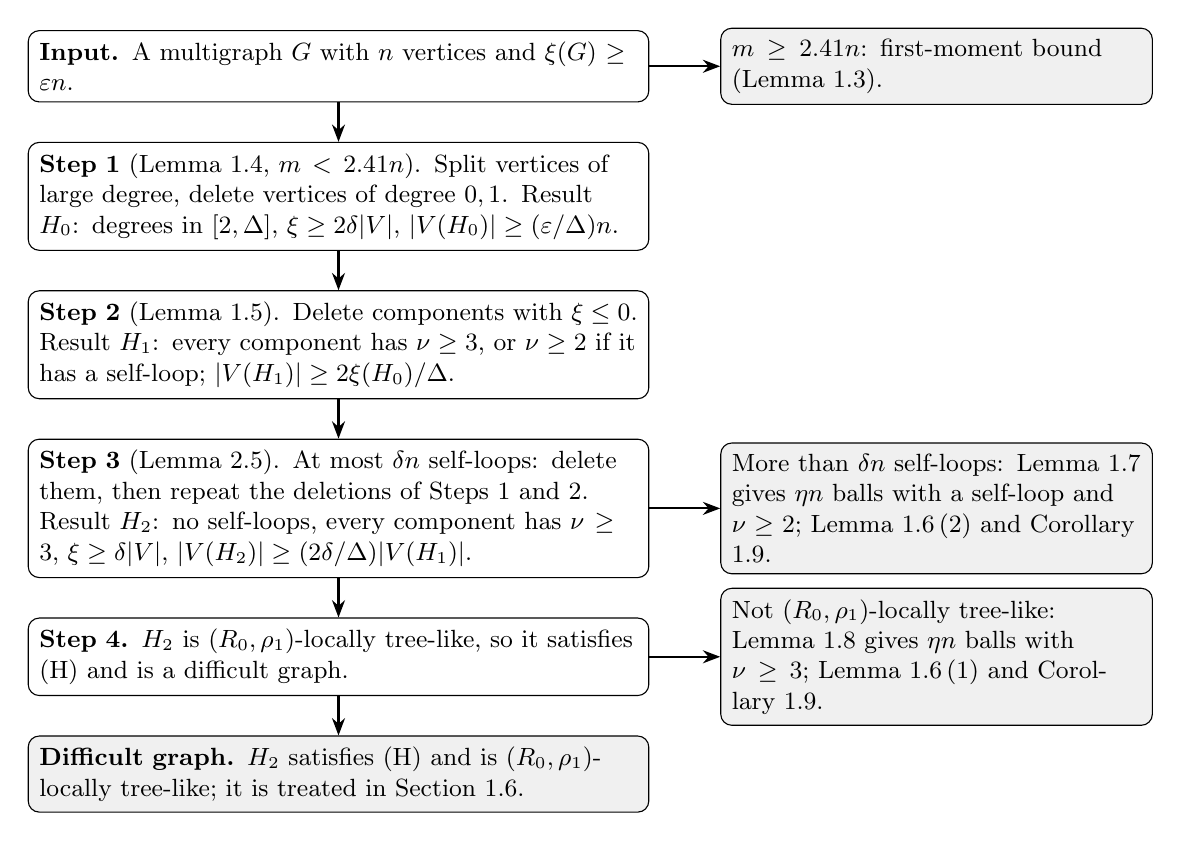
\begin{tikzpicture}[
  node distance=5mm and 9mm,
  stage/.style={draw,rounded corners,align=left,text width=7.6cm,
    inner sep=4pt,font=\small},
  done/.style={draw,rounded corners,align=left,text width=5.2cm,
    inner sep=4pt,font=\small,fill=black!6},
  arr/.style={-{Stealth[length=2.2mm]},thick}]
\node[stage] (in) {\textbf{Input.} A multigraph \(G\) with \(n\) vertices and
  \(\xi(G)\ge\varepsilon n\).};
\node[done,right=of in] (d0) {\(m\ge2.41n\): first-moment bound
  (Lemma 1.3).};
\node[stage,below=of in] (s1) {\textbf{Step 1} (Lemma 1.4, \(m<2.41n\)).
  Split vertices of large degree, delete vertices of degree \(0,1\).
  Result \(H_0\): degrees in \([2,\Delta]\), \(\xi\ge2\delta|V|\),
  \(|V(H_0)|\ge(\varepsilon/\Delta)n\).};
\node[stage,below=of s1] (s2) {\textbf{Step 2} (Lemma 1.5). Delete components
  with \(\xi\le0\). Result \(H_1\): every component has \(\nu\ge3\), or
  \(\nu\ge2\) if it has a self-loop; \(|V(H_1)|\ge2\xi(H_0)/\Delta\).};
\node[stage,below=of s2] (s3) {\textbf{Step 3} (Lemma 2.5). At most
  \(\delta n\) self-loops: delete them, then repeat the deletions of Steps 1
  and 2. Result \(H_2\): no self-loops, every component has \(\nu\ge3\),
  \(\xi\ge\delta|V|\), \(|V(H_2)|\ge(2\delta/\Delta)|V(H_1)|\).};
\node[done,right=of s3] (d3) {More than \(\delta n\) self-loops:
  Lemma 1.7 gives \(\eta n\) balls with a self-loop and \(\nu\ge2\);
  Lemma 1.6\,(2) and Corollary 1.9.};
\node[stage,below=of s3] (s4) {\textbf{Step 4.} \(H_2\) is
  \((R_0,\rho_1)\)-locally tree-like, so it satisfies \Hyp{} and is a
  difficult graph.};
\node[done,right=of s4] (d4) {Not \((R_0,\rho_1)\)-locally tree-like:
  Lemma 1.8 gives \(\eta n\) balls with \(\nu\ge3\);
  Lemma 1.6\,(1) and Corollary 1.9.};
\node[done,text width=7.6cm,below=of s4] (end) {\textbf{Difficult graph.} \(H_2\) satisfies \Hyp{} and is
  \((R_0,\rho_1)\)-locally tree-like; it is treated in Section 1.6.};
\draw[arr] (in) -- (d0);
\draw[arr] (in) -- (s1);
\draw[arr] (s1) -- (s2);
\draw[arr] (s2) -- (s3);
\draw[arr] (s3) -- (d3);
\draw[arr] (s3) -- (s4);
\draw[arr] (s4) -- (d4);
\draw[arr] (s4) -- (end);
\end{tikzpicture}
\end{center}

Steps 1 and 2 keep the excess density \(2\delta\) because Step 3 may lose
\(\delta n\) of the excess when it deletes the self-loops. Self-loops must go
because the main identity (Theorem 1.10) holds only for graphs without
self-loops.

%======================================================================
\section{The deletion experiment (Section 1.5)}\label{sec:experiment}
%======================================================================

The quantities \(K\) and \(T\) in the main identity come from the following
random experiment.

\begin{algorithm}[H]
\caption{Deletion experiment}\label{alg:deletion}
\begin{algorithmic}[1]
\Require a multigraph \(G=(V,E)\) without self-loops, and a fixed order
  \(e_1,\dots,e_m\) of its edges
\State \(F\gets(V,\emptyset)\), \(D\gets\emptyset\)
\For{\(i=1,\dots,m\)}
  \State let \(e_i=uv\)
  \If{\(u\) and \(v\) lie in different components of \(F\)}
    \State flip a fair coin; on heads, add \(e_i\) to \(F\)
  \Else
    \State \(D\gets D\cup\{e_i\}\) \Comment{deferred: its coin is not flipped}
  \EndIf
\EndFor
\State \(T\gets|D|\)
\State \(K\gets\) number of components of \(F\) that contain an edge of \(D\)
\State \Return \(F,T,K\)
\end{algorithmic}
\end{algorithm}

The main identity (Theorem 1.10) is
\(\E\,c(\Sol(\Phi(G)))=\E[2^K(3/4)^T]\). The left side averages over the random
signs, the right side over the coins of the experiment.

%======================================================================
\section{The analysis for difficult graphs (Section 1.6)}\label{sec:difficult}
%======================================================================

\subsection{The bound on \(K\)}

Every component counted by \(K\) contains a cycle of \(G\), formed by a
deferred edge and the path in \(F\) between its endpoints, and different
components give disjoint cycles. This gives
\(K\le(\rho+\frac1{2R})n\) (Lemma 1.13).

\subsection{The bound on \(T\)}

Flip also the coins of the edges in \(D\). Then every edge of \(G\) is kept
independently with probability \(1/2\), so the kept edges form \(G_{1/2}\).
The edges kept in the first stage form the forest \(F\), so every cycle of
\(G_{1/2}\) uses an edge of \(D\), and every outcome satisfies
\(T\ge\nu(G_{1/2})\). It remains to show that \(\E\,\nu(G_{1/2})\) is linear
in \(n\).

For this we compare two ways of reaching the same random subgraph of \(G\).
Going right and then down, we first keep each edge with probability \(1/2\)
and get \(G_{1/2}\), and then keep each of its edges with probability \(p\).
Going along the diagonal, we keep each edge of \(G\) with probability \(p/2\)
in one step. Both routes keep every edge independently with probability
\(p/2\), so they give the same law.

\begin{center}
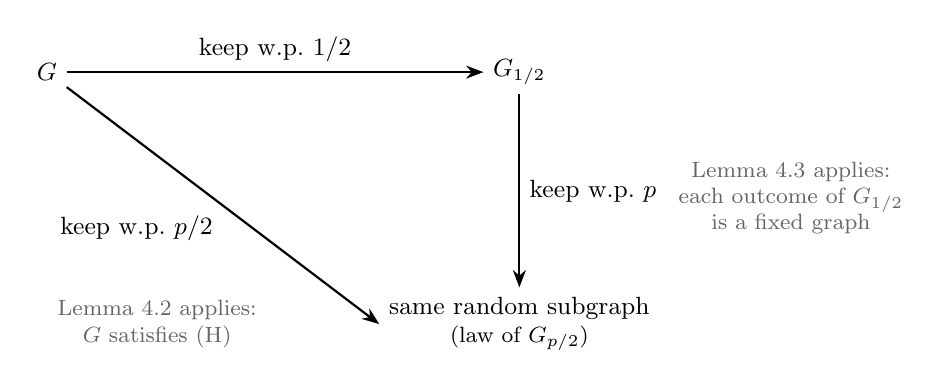
\begin{tikzpicture}[
  every node/.style={font=\small},
  arr/.style={-{Stealth[length=2.2mm]},thick},
  note/.style={font=\footnotesize,text=black!60,align=center}]
\node (G) at (0,0) {\(G\)};
\node (F) at (6,0) {\(G_{1/2}\)};
\node[align=center] (Z) at (6,-3.2) {same random subgraph\\[-1pt]
  {\footnotesize(law of \(G_{p/2}\))}};
\draw[arr] (G) -- node[above] {keep w.p.\ \(1/2\)} (F);
\draw[arr] (F) -- node[right] {keep w.p.\ \(p\)} (Z);
\draw[arr] (G) -- node[below left] {keep w.p.\ \(p/2\)} (Z.west);
\node[note,anchor=west] at (7.9,-1.6) {Lemma 4.3 applies:\\ each outcome of
  \(G_{1/2}\)\\ is a fixed graph};
\node[note] at (1.4,-3.2) {Lemma 4.2 applies:\\ \(G\) satisfies \Hyp};
\end{tikzpicture}
\end{center}

Since the two routes give the same law,
\(\E[\Lp_\ell(G_{1/2},p)]=\Lp_\ell(G,p/2)\). Lemma 4.3 bounds the left side
from above for each outcome of \(G_{1/2}\), and Lemma 4.2 bounds the right side
from below. With \(p=p_0\), \(\ell=\ell_0\) and \(\kappa=\zeta/2\) this gives
\[
  \zeta
  \le\Lp_{\ell_0}(G,p_0/2)
  =\E\bigl[\Lp_{\ell_0}(G_{1/2},p_0)\bigr]
  \le\frac\zeta2+2M_{\ell_0}\frac{\E\,\nu(G_{1/2})}{n},
\]
so \(\E\,\nu(G_{1/2})\ge\omega n\) with \(\omega=\zeta/(4M_{\ell_0})\)
(Lemma 4.4). The factor \(1/2\) comes from the deletion experiment, and this is
why Lemma 4.2 is stated for the retention probability \(p_0/2\). A
bounded-differences inequality then turns this bound on the expectation into
\(\E[(3/4)^T]\le2e^{-\gamma n}\) (Lemma 1.14).

\subsection{Order of the constants}\label{sec:constants}

Each line uses only the constants on the lines above it.

\begin{enumerate}[label=(\arabic*)]
\item \(\varepsilon\) is given.
\item Lemma 1.4: an integer \(\Delta>2+5/\varepsilon\) and
  \(\delta=\varepsilon/(4(1+\varepsilon))\). From now on \(\Delta,\delta\) are
  fixed.
\item Appendix A: \(\lambda=2(1+\delta)^{1/4}\in(2,2(1+\delta))\),
  \(\mu=\log(2(1+\delta))-\log\lambda\), \(U=\log(\Delta-1)\),
  \(\psi=\mu^2/(32U^2)\), and \(\rho_0\) with \(\Delta\rho_0/2\le\psi\).
\item Lemma 4.2: \(p_0=\frac12(2/\lambda+1)\in(2/\lambda,1)\) and
  \(\zeta=\frac{2\psi^2}{\Delta}\bigl(1-(\tfrac{p_0}2\lambda)^{-1}\bigr)\).
\item Lemma 4.4: \(\ell_0\) from Lemma 4.3 with \(p=p_0\), \(\kappa=\zeta/2\),
  and \(\omega=\zeta/(4M_{\ell_0})\).
\item Lemma 1.14: \(\gamma=\min\{\tfrac\omega2\log\tfrac43,\ \omega^2/\Delta\}\).
\item Theorem 1.12: \(R_0=\max\{\ell_0,\lceil2\log2/\gamma\rceil\}\) and
  \(\rho_1=\min\{\rho_0,\ \gamma/(4\log2)\}\).
\item Section 4.7: Lemma 1.7, called with \((\Delta,\delta)\), gives \(R_1\) and
  \(\eta=\delta/\Delta\). Lemma 1.8, called with \((\Delta,R_0,\rho_1)\), gives
  \(R_1=2s+R_0\) and \(\eta=\rho_1/(8M_{2R_0})\). Corollary 1.9 is called with
  these \((\Delta,R_1,\eta)\).
\end{enumerate}

The key point is line (6): \(\gamma\) depends only on \(\Delta,\delta\), and not
on \(R,\rho\). So \(R,\rho\) can be chosen last, with
\((\rho+\tfrac1{2R})\log2\le\gamma/2\), and then the factor
\(2^K\le2^{(\rho+1/(2R))n}\) is beaten by \(\E[(3/4)^T]\le2e^{-\gamma n}\).

\end{document}
